\section{Evaluation}
\label{sec:evaluation}

Because \Syndicate\ is storage middleware,
it is on the critical path for reads and writes.
We focus on quantifying the I/O overhead
\Syndicate\ introduces on top of directly leveraging 
the underlying infrastructure.  The common theme in our evaluation is
to measure the systemic performance 
for a particular set of operations, and then break down
where time was spent---how much in \Syndicate, and
how much in the underlying infrastructure.  We do so by 
examining the {\it relative} performance of \Syndicate\
on top of controlled infrastructure, compared to directly 
accessing data.  We show that a large
fraction of I/O overhead can be reduced simply 
by leveraging better infrastructure, validating the need 
for our system.

Due to its immediate applicability to PlanetLab users,
we focus on evaluating the peer-to-peer deployment model.
This extends to understanding the performance of our example
applications---the scientists' workstations, the document servers, and 
VDI VM servers all run both a User \SGs\ and Replica \SGs\ to 
process, store, and serve data to one another across 
the wide-area.

\subsection{Testbed}

We selected 300 PlanetLab nodes with the shortest {\tt ssh} connection times,
and provisioned a User \SG\ and Replica \SG\ on each.  The User \SG\
leveraged a local Squid~\cite{Squid} cache to store recently-read block and
manifest data.  We varied the 
behavior of the Replica \SG\ depending on what we needed to measure.

We built a CDN from Squid~\cite{Squid} caches on top of
40 VICCI~\cite{VICCI} nodes distributed evenly across the
four North American sites.  We used the Aura request router~\cite{aura-rr}
(based on~\cite{cdn-redirect}) with a variant of consistent hashing
to distribute a client request to one of three VICCI nodes, based
on the client IP address.

The PlanetLab caches were configured to use 256MB of RAM and 1GB of disk.
The VICCI caches were configured to use 1GB of RAM and 8GB of disk.  These sizes 
were chosen to be big enough to store our working set, so as to consistently
measure the performance of hitting partially-cached object data.
In addition, PlanetLab nodes were limited to 10Mbps maximum bandwidth 
and 10GB maximum data sent per day.

We set up the \MS\ with the configuration we plan to offer users
(others are possible, at different price-points).  Each \MS\ instance
in Google AppEngine had a 1GHz virtual CPU and 512MB RAM.  We used the
High Replication Datastore (HRD) for storing and replicating \MS\
records (where individual record replication is coordinated via
Paxos~\cite{paxos}).  We allocated 50 static instances, and
allowed Google to start more automatically.

\subsection{Metadata Operations}

% compare metadata operation time to no-op GET that involves reading something out of ndb
% (can look this up on Google in the worst-case)

While a scalable number of \SGs\ read
and write a scalable number objects,
each \SG\ contends with an interactive workload.
Since each \SG\ communicates with the \MS\ as part of its control plane,
the choice of \MS\ platform will influence \Syndicate's overhead.

To understand how, we measured the time taken by a metadata operation
between the call into the \MS\ client library
and its return.  This includes the added latency
from the \MS\ platform, which we measure indirectly by 
measuring the time taken by our \MS\ code to process a request.

We simulated a set of peer \SGs\
managing a peer-specific directory of peer-specific objects, which 
is a common access pattern for our sample applications.
We first had each \SG\ create
a top-level directory in the Volume (``Mkdir''), forcing the \MS\ to serialize
many directory writes at once.  We then had each \SG\ create an object within
this directory (``Create''), where no serialization is required.  Afterwards,
each \SG\ wrote new metadata for the object (``Update'') and then redownloaded all 
metadata for its path (``Revalidate'').  Finally, each \SG\ deleted the object
(``Unlink'') and then its parent directory (``Rmdir'').

We started each \SGs\ in a staggered fashion, so as to 
maximize churn in the \MS.  Each \SG\ used a keep-alive
HTTPS connection to issue the requests; the latency of the initial
SSL negotiation is omitted (since it is noticed only when the \SG\ registers 
with the \MS).  The runtimes are summarized in Figure~\ref{fig:metadata-latency}.


\begin{figure}[h!]
\centerline{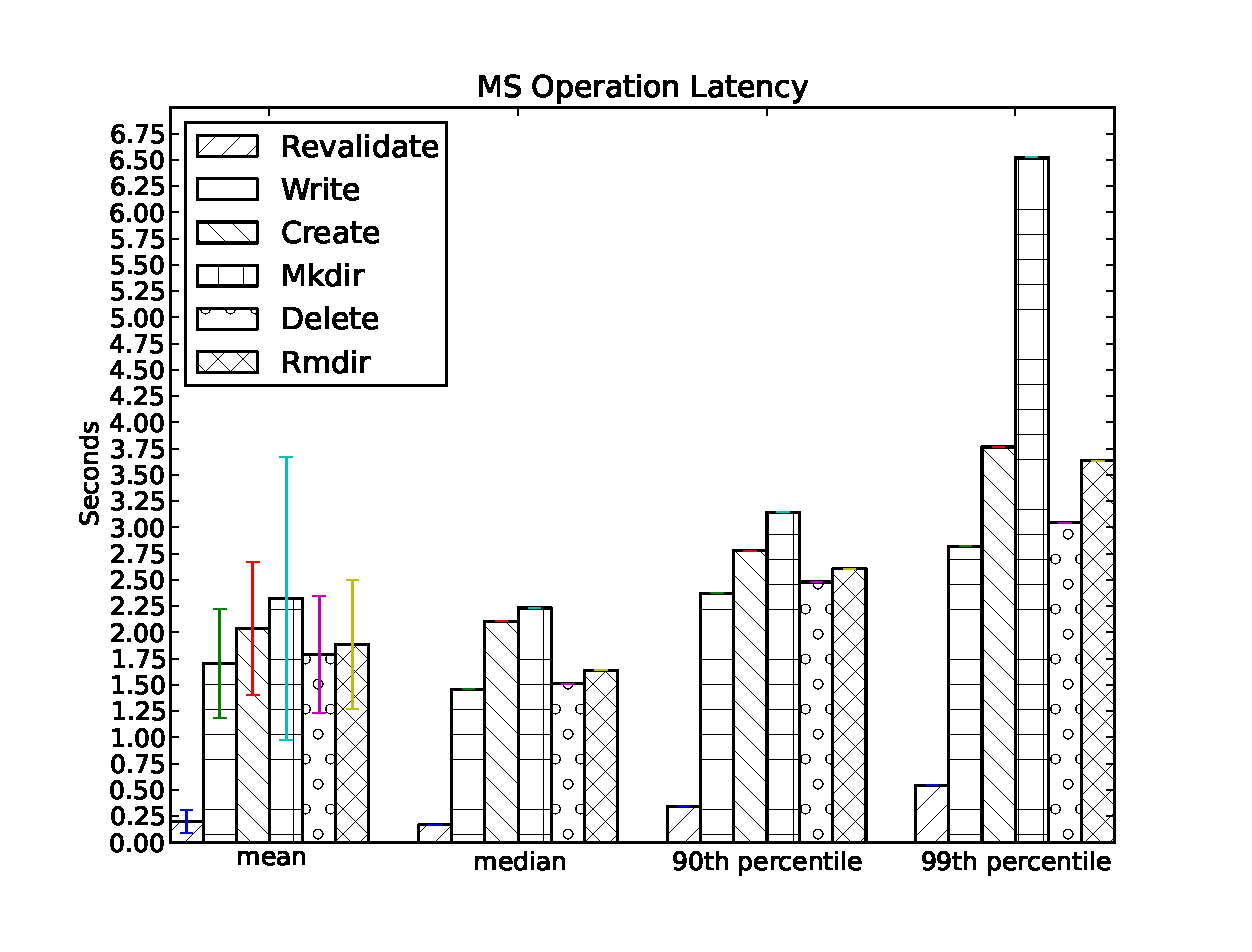
\includegraphics[width=0.55\textwidth]{figures/metadata_operations}}
\caption{\it 
Metadata operation times (in seconds) across 300 PlanetLab nodes.  Error bars are one standard deviation.}
\label{fig:metadata-latency}
\end{figure}

In addition, we recorded Google AppEngine's self-reported
performance for the API calls we leverage~\cite{google-appengine-status}.
Their performances, as well the number of times each \MS\ operation uses them,
are summarized in Table~\ref{tab:gae-performance}.  Note that a datastore {\tt get} 
is called whenever a memcache {\tt get} fails.

\begin{table*}[ht!]
\begin{tabular}{ | l | l | l | l | l | l | l |}
\hline
\textbf{Operation} & \textbf{Min (ms)} & \textbf{Max (ms)} & \textbf{Create/Mkdir} & \textbf{Revalidate} & \textbf{Update} & \textbf{Unlink/Rmdir} \\
\hline
datastore {\tt get}    & 35  & 65  & 0-2 & 0-1 & 0-1 & 0-2 \\
datastore {\tt put}    & 45  & 70  & 1   & 0   & 1   & 3 \\
datastore {\tt update} & 50 & 120  & 1   & 0   & 0   & 0 \\
datastore {\tt query}  & 80 & 150  & 0   & 0-1 & 0   & 0-1 \\
memcache {\tt get}     & 1  & 10   & 4   & 2   & 2   & 3 \\
memcache {\tt set}     & 2  & 10   & 4   & 2   & 3   & 6 \\
HTTPS {\tt GET}        & 25 & 100  & 1   & 1   & 1   & 1 \\
\hline
\end{tabular}
\caption{\it Approximate (self-reported) min/max latency from Google AppEngine on
API calls, and the numbers of each API method synchronously
called by each \Syndicate\ metadata operation. The {\tt update}
operation is a transaction of one {\tt get} and one {\tt put}. }
\label{tab:gae-performance}
\end{table*}

Using the AppStats~\cite{gae-appstats} middleware,
we confirmed that each operation ran
at least as slowly as the minimum
times indicated by GAE's self-reporting.
Additionally, we observed that most of the latency of each
operation (particularly higher percentiles) was due to GAE buffering our 
requests internally---GAE holds a request for up to 
10s before allowing a tenant to process it.  The reason
``Revalidate'' operations are so short relative to the 
rest is because most of the time, it only interacts with 
{\tt memcache}, making it a much faster operation.

While we can improve \MS\ performance by using a lower-latency platform,
making namespace updates atomic in ``Create'' is
nevertheless a costly but necessary operation.
Regardless, the \MS\ is able to deliver metadata 
to readers quickly enough for interactive workloads even under 
degenerate conditions-- -when the \SG\ has not 
cached any metadata, when there is a high buffering time in the provider,
and when there is a lot of churn in the directory structure.
This is adequate for our sample applications.

\subsection{Reads and Consistency}

To evaluate \Syndicate's overhead for reading consistent data,
we had each VM create and then read a 6MB object
comprised of 100 60KB blocks.
We chose this object size to make it sufficiently 
large to merit distribution by CDN, and chose 100 blocks 
to generate a large number of GET requests at once (30,000 blocks and 300 manifest 
requests, or about 2GB of data, per experiment).  In the context of our sample applications,
a single object represents a piece of experimental data, a large document, or
a VM's session information.

In these experiments, object data was stored on local
disk on each VM and and read sequentially by the User \SG.  Due to
its similarity to
the Replica and Acquisition \SGs\ in
processing reads (beyond evaluating a specific $R$ function), the 
insights into its overhead extend to understanding
the the other two \SGs' read overheads.

{\bf Read Latency.} To understand \Syndicate's overhead for accessing data,
we measured read latency for reading the object sequentially, from
both local and remote \SGs.  We defined latency as the wall-clock time between 
entering the call to {\tt read()} and the receipt of the first byte 
of object data in the \SG, in order to account for all the overhead of 
preparing to receive data (namely, revalidating the object metadata and 
downloading a fresh manifest).  To ensure the \SG\ did not falsely
report zero latency on remote reads, we used cold caches and had each \SG\ choose a
remote object at random to read.

The local read latencies for the \SGs\ are summarized
in Figure~\ref{fig:read_latency_local}, and 
the remote read latencies in Figure~\ref{fig:read_latency_remote}.  In the local case,
there is no appreciable latency difference between reading local data through
\Syndicate\ (``Read, local object'') and reading 100 60KB local files directly (``Read, disk'').
Almost all of the overhead comes from revalidating the object's metadata first
(``Read, local object + Revalidate'').

\begin{figure}[h!]
\centerline{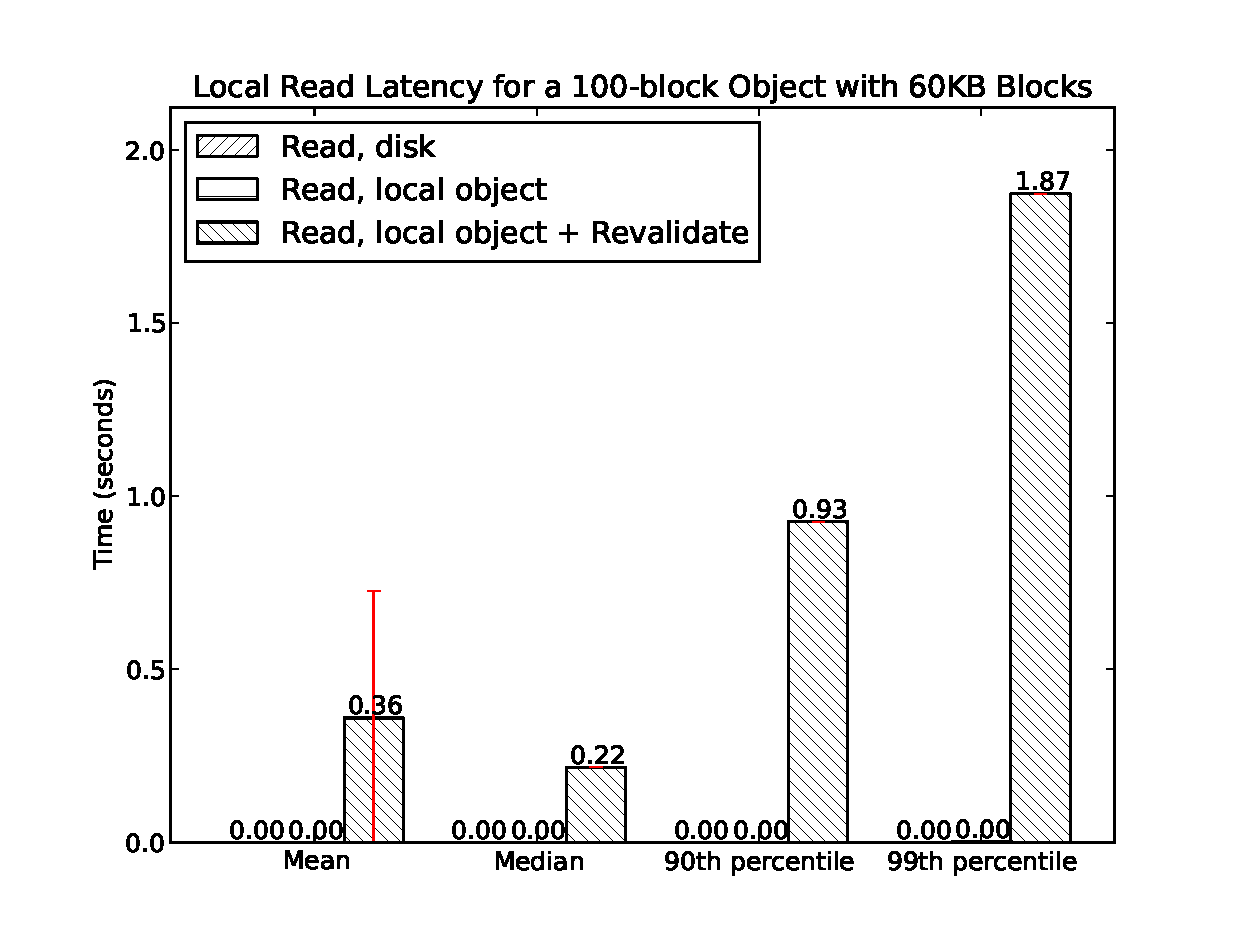
\includegraphics[width=0.55\textwidth]{figures/read_latency_local}}
\caption{\it Read latencies on a local object's data.  Error bars are one standard deviation.}
\label{fig:read_latency_local}
\end{figure}


\begin{figure}[h!]
\centerline{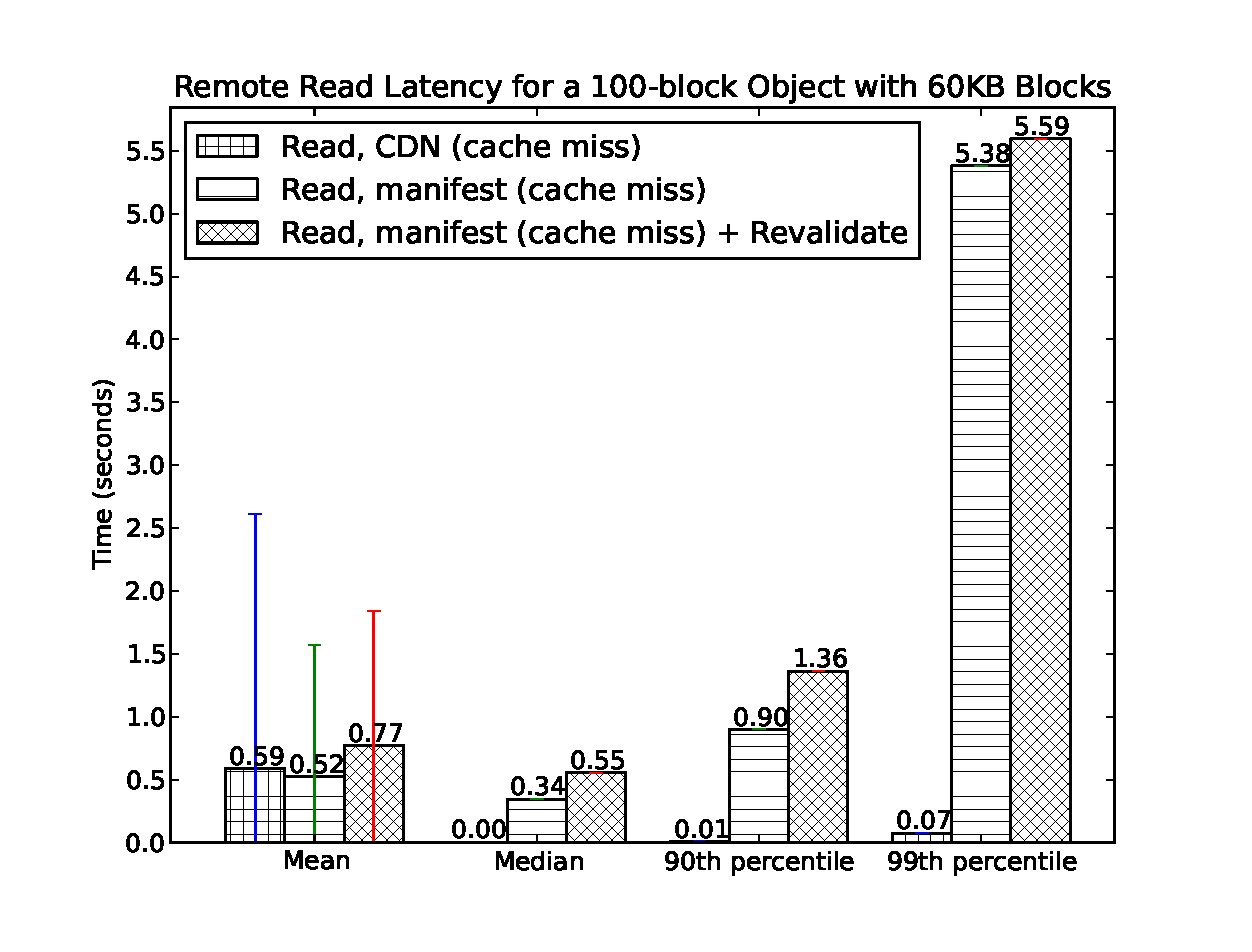
\includegraphics[width=0.55\textwidth]{figures/read_latency_remote}}
\caption{\it Read latencies on a remote object's data.  Error bars are one standard deviation.}
\label{fig:read_latency_remote}
\end{figure}

In the remote case, the \SG\ first downloaded the manifest before reading 
the object data.  We compare the latency added by downloading the manifest only
(``Read, manifest (cache miss)'') to the latency added by downloading the
manifest and also refreshing the object 
metadata (``Read, manifest (cache miss) + Revalidate'').  As a baseline comparison,
we additionally measured latency added just by contacting the CDN for object data
(``Read, CDN (cache miss)'').

We see that the latency added by the CDN
is very small---70ms in the 99th percentile---and that most of
the overall latency comes from fetching the manifest on cache miss.  However, a
local \SG\ evaluation shows that it can generate and parse responses
for manifest requests much more quickly than this test indicates, suggesting that the underlying 
infrastructure---the wide-area network and PlanetLab VMs---contributes most of the 
latency, and that replacing it with faster infrastructure would reduce it.

{\bf Read Times.} We measured the read time for the
object on each \SG\ as the wall-clock time elapsed
between receiving the first and last byte of data, after the manifest and 
metadata had been downloaded.  We used both cold and warm caches on remote 
reads, to compare the worst-case performance (local and CDN cache miss) to the best-case
(local and CDN cache hit).  To serve as a baseline comparison for remote reads in both cases,
we used the {\tt curl} program to download the same 100 60KB blocks.  
With both {\tt curl} and the \SG, each block was fetched sequentially and as separate requests.

The results are summarized in Figure~\ref{fig:read_performance} (note the logarithmic time 
axis).  Unsurprisingly, reading all 100 60KB blocks of a local object on the
\SG\ (``Read, local object'') and directly reading them (``Read, disk'')
are comparable, with \Syndicate\
adding 30ms extra time in the 99th percentile.

\begin{figure*}
\centerline{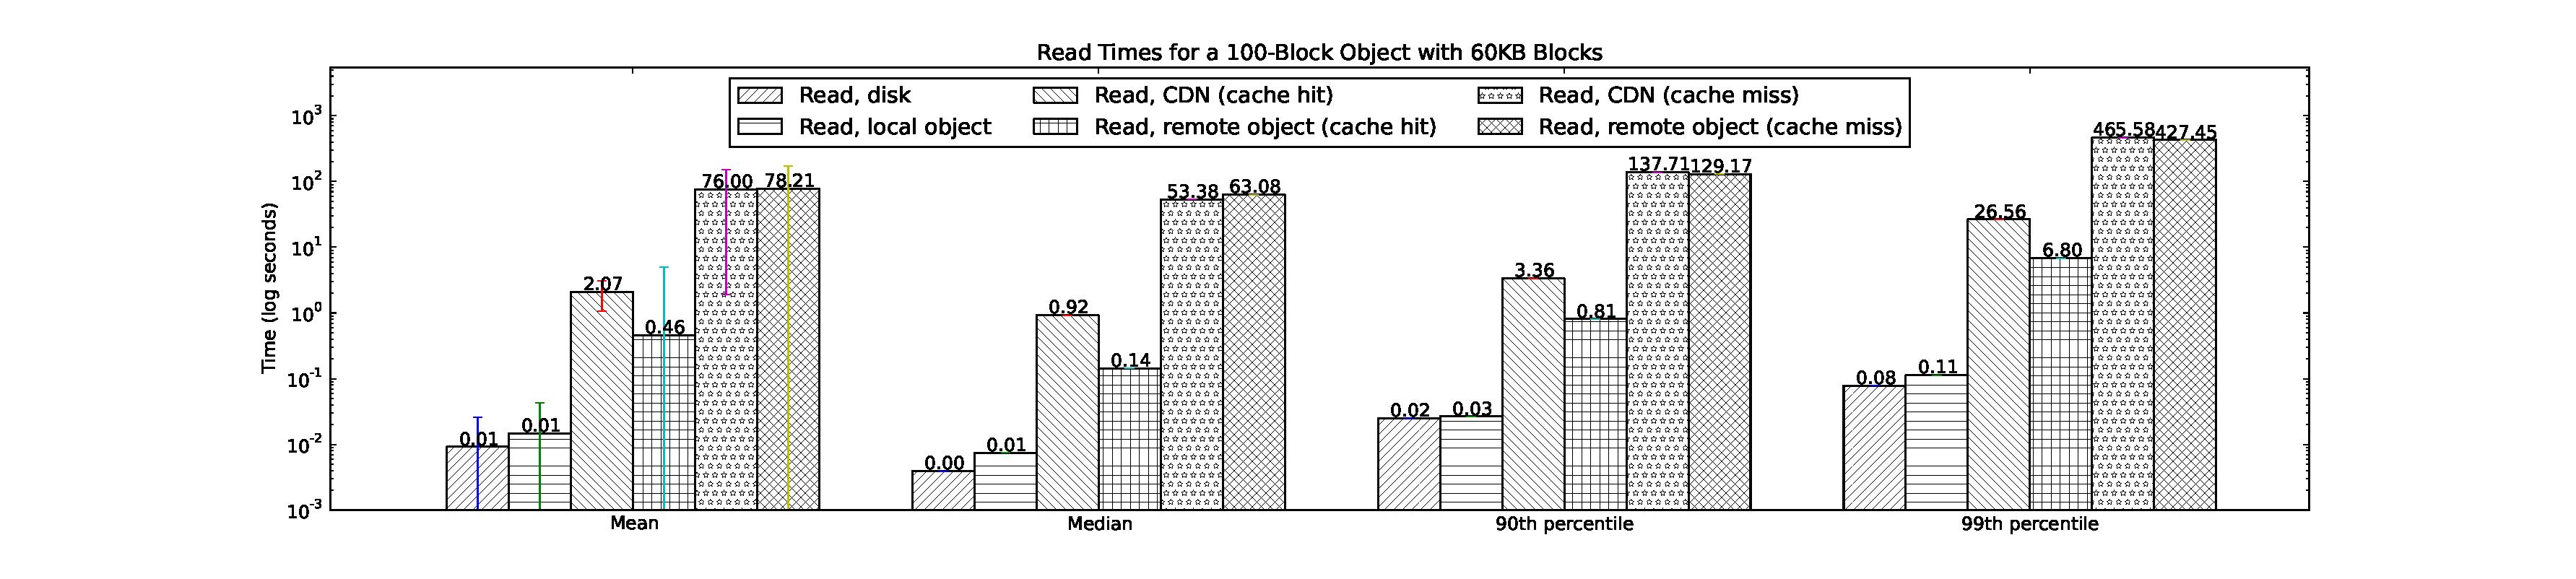
\includegraphics[width=1.2\textwidth]{figures/read_performance}}
\caption{\it
Read times of \Syndicate, as compared against reading blocks directly from disk and directly from the CDN (on both cache hit and miss).  Note that the Y axis is in log-scale.  Error bars are one standard deviation.  Numbers on each bar are in seconds.}
\label{fig:read_performance}
\end{figure*}

However, the \SG\ was consistently faster than {\tt curl} when reading locally-cached block data
(``Read, CDN (cache hit)'' versus ``Read, Remote Object (cache hit)'').  This was 
due to the slowdown added by running the {\tt curl} program once for each block, whereas
the \SG\ used {\tt libcurl} to sequentially fetch blocks and thus benefitted from
preserving library state across requests.  Specifically, most of the
difference was from reusing cached DNS queries.

This time difference is also visible when reading block data through cold caches
(``Read, CDN (cache miss)'' versus ``Read, remote object (cache miss)''), and 
is consistent with the difference observed when reading cached data.
This suggests that read bandwidth of the \SG\ versus {\tt curl} is otherwise
comparable, and indicates that the CDN was the limiting factor to read times.

{\bf Reads with Writes.}  To demonstrate the overall
effect of reading data after it is written, we 
had 299 \SGs\ concurrently read the 300th \SG's object after a controlled
percentage of its blocks were overwritten.  After a write, each remote \SG\ downloaded 
the new metadata and manifest, and sequentially read all of the object's blocks
from warm caches.  We warmed the caches prior to the first write by having each \SG\ 
read the object's blocks.  We also disabled cache control directives, requiring 
the local caches and CDN to keep data indefinitely.


\begin{figure}[h!]
\centerline{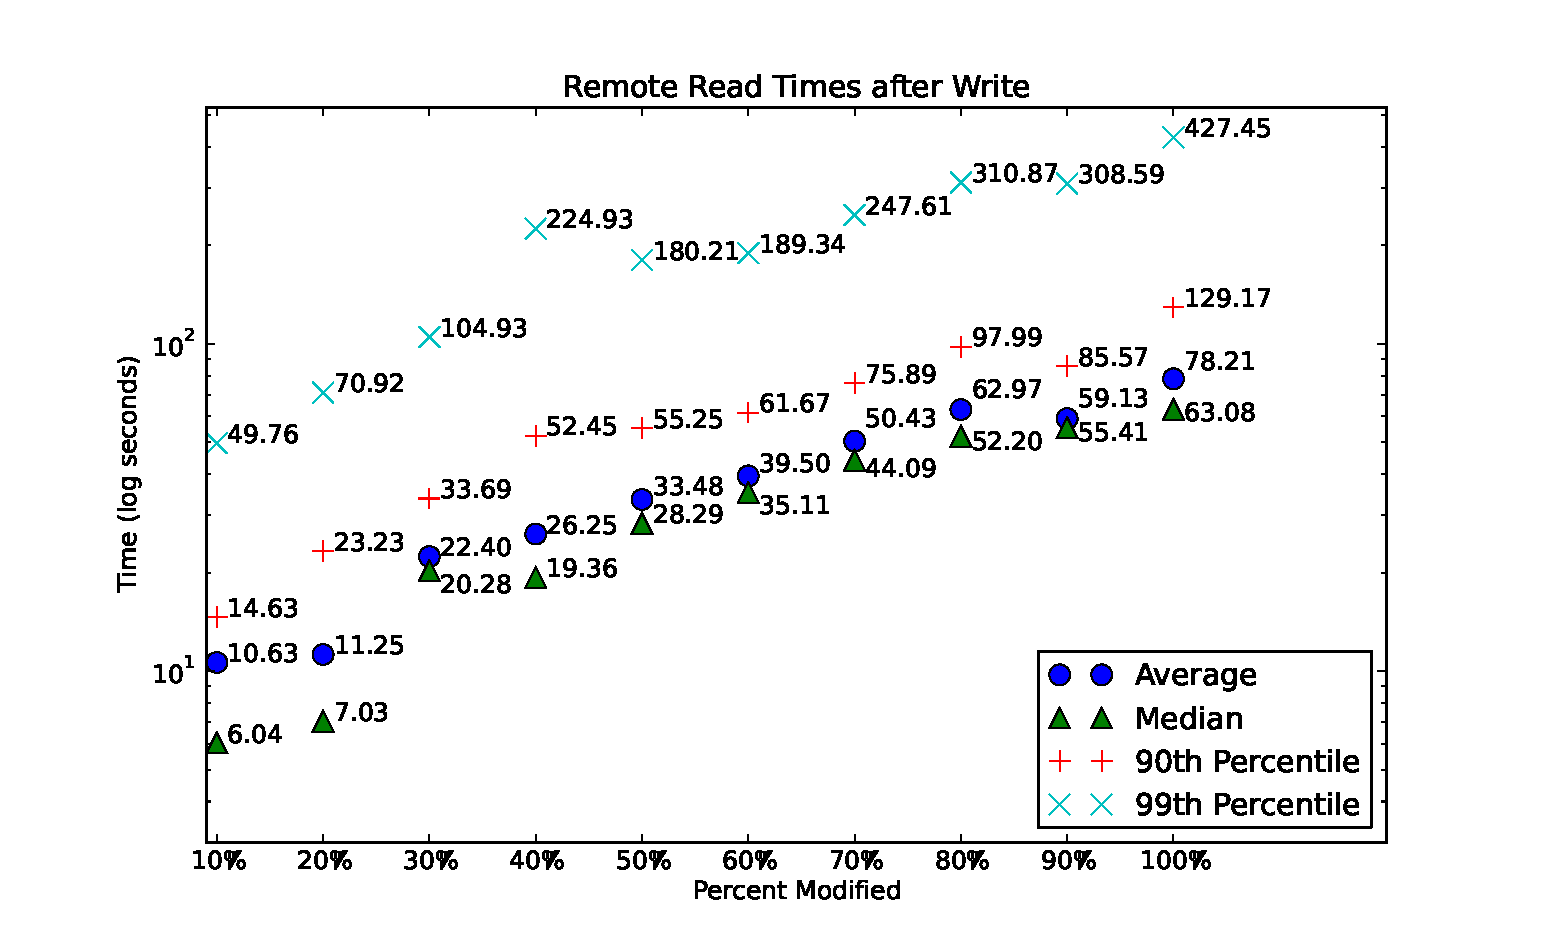
\includegraphics[width=0.55\textwidth]{figures/read_after_write}}
\caption{\it Times taken to read a remote object after a given percent of its blocks were modified.  Note that the Y axis is in log-scale.}
\label{fig:read_after_write}
\end{figure}

We overwrote the object in 10\% increments, and measured
the total time to read the object as the wall-clock time between the application 
calling {\tt read()} and {\tt read()} returning.  The times are summarized
in Figure~\ref{fig:read_after_write}.

Predictably, there is a roughly linear correlation between the fraction of modified 
blocks and the total read time, in all percentiles.  This validates the benefit of breaking 
objects into chunks in the storage layer, and managing consistency separately from 
data locality---readers hit unmodified data in the cache and redownload modified data
automatically, without needing cache control directives.


\subsection{Writes and Consistency}

To measure how much overhead writes introduce, we measured the time 
taken to write all the object data to local disk (``Write, local object''), as well as the time
taken to additionally send a new last-write nonce to the \MS\ (``Write + MS update'').
We compared both scenarios to simply writing
100 60KB files to disk (``Write, disk'').  The results are summarized in 
Figure~\ref{fig:write_performance}.


\begin{figure}[h!]
\centerline{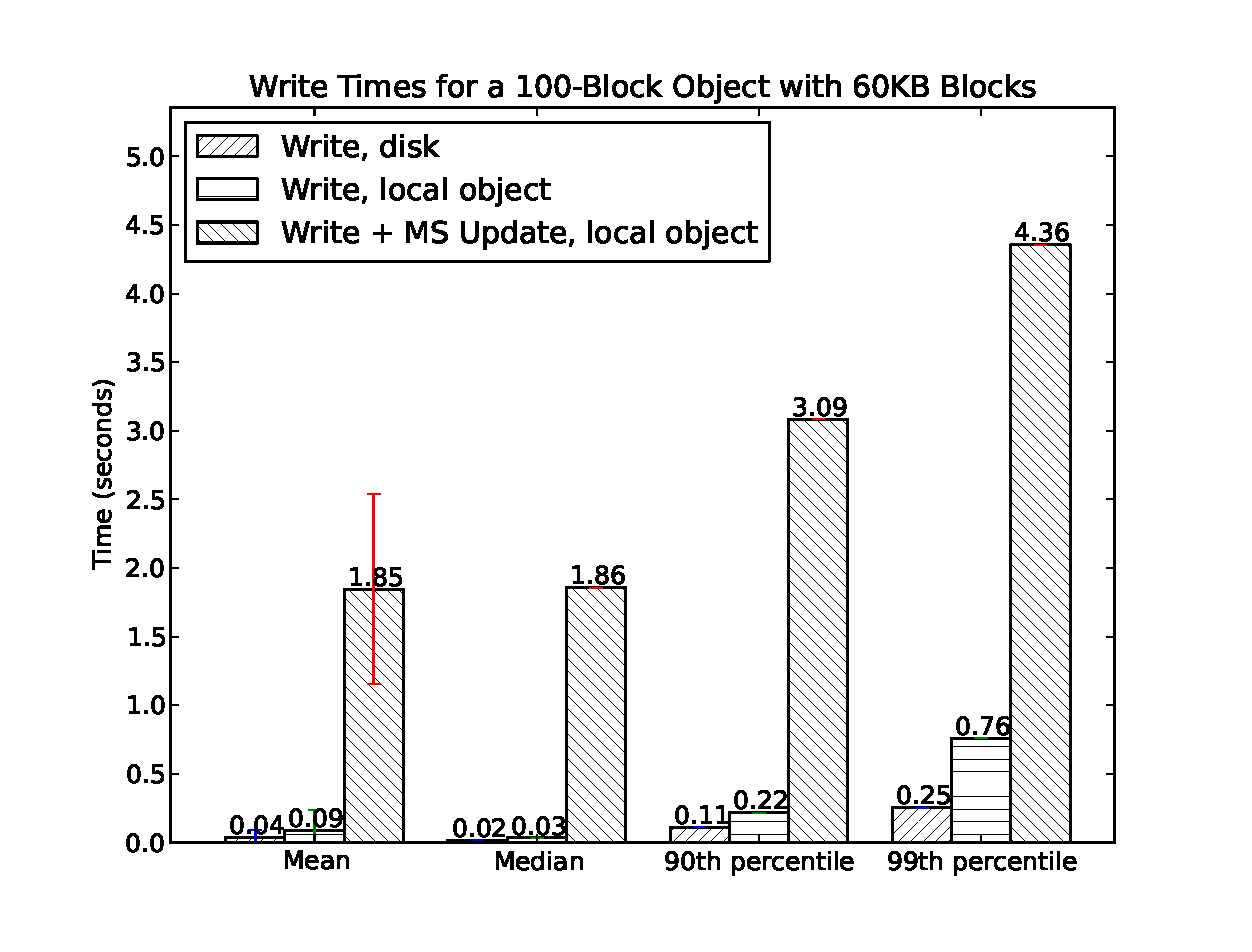
\includegraphics[width=0.55\textwidth]{figures/write_performance}}
\caption{\it Times taken to write a local object's data.  Error bars are one standard deviation.}
\label{fig:write_performance}
\end{figure}

In comparing writing directly to disk to writing to the \SG, we observe that \Syndicate\
adds a 3x write overhead in the 99th percentile, but a 1.5x overhead in the 50th
percentile.  This is due to two factors:  keeping the manifest up-to-date with 
written data, and preserving some extra state on disk to track the last-write nonce.
Both of these routines are not yet optimized in our \SG\ prototype.  Nevertheless,
the cost of updating the last-write nonce on the \MS\ dominates the cost to write 
this object.

\subsection{Discussion}

While this is a preliminary evaluation, we believe it provides enough
information to demonstrate that \Syndicate\ not only works, but also
that our example applications (and others) could benefit by using it
in read-heavy but read-write interactive workloads.

One take-away is that the choice of infrastructure plays a big role
in determining \Syndicate's performance.  This is by design, because
the performance benefits a provider can offer should be passed on to
the application whenever possible.

We are in the process of deploying \Syndicate\ as a permanent service
in PlanetLab, such that users will automatically receive one Volume per
slice, and each VM will automatically install and mount our FUSE \SG.
Our full running system will leverage a private
instance of the CoBlitz~\cite{coblitz} CDN deployed on VICCI.  We will
maintain a set of Replica \SGs\ for
popular cloud storage providers, which users may choose when creating
their Volumes.

